\documentclass[10pt,journal,twocolumn,twoside]{IEEEtran}
\usepackage{amsmath,amssymb,amsfonts,float}
\usepackage{graphicx,bm,psfrag,amsmath,enumitem,amsthm}
\def\mmax{\mathop{\mbox{\scriptsize max}}}
\def\argmin{\mathop{\mbox{arg\,min}}}
\def\argmax{\mathop{\mbox{arg\,max}}}
\newcommand{\defequal}{\stackrel{\mathrm{def}}{=}}
\renewcommand{\vec}[1]{{\ensuremath{\boldsymbol{#1}}}}
\newcommand{\popt}{\ensuremath{P^{(K)}_{opt}}}
\pagestyle{plain}
\usepackage{algorithm, algorithmic}
\renewcommand{\algorithmicrequire}{ \textbf{Input:}} %Use Input in the format of Algorithm
\renewcommand{\algorithmicensure}{ \textbf{Procedures:}} %UseOutput in the format of Algorithm
\newtheorem{mypro}{Proposition}
% correct bad hyphenation here
%\hyphenation{op-tical net-works semi-conduc-tor}
\usepackage{CJK}
\usepackage{color}
\usepackage{url}
\usepackage{geometry}
\geometry{left=0.6in, right=0.6in, top=0.75in, bottom=0.75in}
\def\BibTeX{{\rm B\kern-.05em{\sc i\kern-.025em b}\kern-.08em
    T\kern-.1667em\lower.7ex\hbox{E}\kern-.125emX}}

\begin{document}

\title{Jointly Digital Precoding and Power Allocation for BDMA Downlink Transmissions by Rank-constrained D.C. Programming}
\author{\IEEEauthorblockN{Guanchong Niu, Qi Cao, Man-On Pun\IEEEauthorrefmark{3}\\
		\IEEEauthorblockA{
			The Chinese University of Hong Kong, Shenzhen\\
			Guangdong, China, 518172
			\thanks{This work was supported, in part, by the CUHKSZ President's Fund under Grant No. PF.01.000211, the Shenzhen Science and Technology Innovation Committee under Grant No. ZDSYS20170725140921348 and the National Natural Science Foundation of China under Grant No. 61731018.} \thanks{\IEEEauthorrefmark{3} Corresponding author, email: SimonPun@cuhk.edu.cn.}
}}}
\maketitle\thispagestyle{plain}\pagestyle{plain}

\begin{abstract}
Beam Division Multiple Access (BDMA) with hybrid precoding has recently been proposed for multi-user multiple-input multiple-output (MU-MIMO) systems by simultaneously transmitting multiple digitally precoded users' data streams via different beams. In the hybrid precoding system, the analog and digital precoder design as well as the power allocation problem are highly non-convex. In this paper, we first solve the analog precoder by exhaustively searching the feasible sets by assuming orthonormal digital precoders. After obtaining the analog precoder, the non-convex problem can be reformulated as an iterative rank-constrained D.C. (difference of two convex functions) programming problem by setting a dummy variable. Distinct from the conventional heuristic algorithms like zero-forcing, balanced-SINR (Signal-to-interference-and-noise ratio) or max-SLNR (Signal-to-leakage-and-noise ratio) precoders, the proposed algorithm directly maximizes the weighted rate $\tau_u\log_2(1+\text{SINR}_u)$ of $u$-th user instead of interference or leakage alone. Furthermore, the iterative algorithm is proved to be monotonic and convergent. The simulation results confirm the effectiveness and convergence of the proposed iterative algorithm.
\end{abstract}

%\begin{keywords}
%BDMA, Hybrid Beamforming, Block Diagonal Precoder, PAPR, User Scheduling.
%\end{keywords}

\begin{IEEEkeywords}
	BDMA, Hybrid Beamforming, D.C. Programming, Power Allocation.
\end{IEEEkeywords}

%\titlepgskip=-15pt

%\maketitle

\section{Introduction}\label{sec:introduction}
To meet the ever-increasing demand of higher user data rates, it is envisioned that the next-generation cellular systems will be equipped with massive antenna arrays. Capitalizing on a large number of antennas at the base station (BS), Beam Division Multiple Access (BDMA) has recently been proposed to transmit multiple users' data-streams via different beams. In contrast to the more conventional multiple access schemes such as Code Division Multiple Access (CDMA) or Orthogonal Frequency Multiple Division Access (OFDMA) that multiplex users in code, time and frequency domains, BDMA separates users in the beam space by transmitting data to different users in orthogonal beam directions. In \cite{sun2015beam}, BDMA was first proposed to decompose the multiuser multiple-input multiple-output (MU-MIMO) system into multiple single-user MIMO channels by multiplexing multiple users' data onto non-overlapping beams. BDMA is particularly attractive in practice as beamforming is commonly implemented in the analog domain using low-cost phase shifters. More recently, joint user scheduling and beam selection for BDMA was formulated under the Lyapunov-drift optimization framework before the optimal user-beam scheduling policy was derived in a closed form \cite{Jiang2018}. However, the assumption of non-overlapping orthogonal beams is hard to be satisfied. As a result, the inter-user interference caused by the non-orthogonality between beams has handicapped the analog-only BDMA applications.

In the meantime, digital precoding has been well studied as an effective signal processing means to control residual interference for MU-MIMO. The classical fully digital precoding requires a dedicated radio frequency (RF) chain for each antenna. Since RF chains are expensive, fully digital precoding has become impractical for massive MIMO systems. To overcome this obstacle, hybrid digital and analog beamforming has been proposed for massive MIMO transmissions by dividing the precoding process into two steps, namely analog and digital precoding. More specifically, the transmitted signals are first precoded digitally using a smaller number of RF chains followed by the analog precoding implemented with a much larger number of low-cost phase shifters. As a result, the hybrid analog-digital precoding architecture requires significantly less RF chains as compared to the fully digital precoding. It has been reported in the literature that the hybrid beamforming structure is capable of achieving performance comparable to the fully digital beamforming scheme if the number of RF chains at each end is greater than or equal to twice the number of the data streams \cite{han2014reference}. Therefore, the hybrid precoded massive MIMO system can benefit from the interference suppression provided by the digital precoding while harvesting large antenna beamforming gains by exploiting the massive antennas available in the systems. This hybrid structure is particularly attractive for millimeter wave (mmWave) MIMO systems to support Gbps-order data throughput by exploiting the vast vacant spectrum available at RF of $6$ GHz or above.

Despite the advantages for hybrid beamforming structure, the analog and digital precoders are intractable to be designed in closed-form since its non-convexity and complexity.  
Besides, Power allocation is also an important problem in co-channel interference management for the multi-users wireless network. Since the objective function is highly non-convex, the computation for global optimal solutions is usually very difficult and complicated, especially for the coupled analog and digital precoding constraints. Therefore, most of the existing works considered the precoder and power allocation problems separately. \cite{sohrabi2016hybrid} alternatively optimizes the power allocation for sum-rate capacity maximization problem implementing water filling by assuming the analog precoders are strictly orthogonal among distinct users, \textit{i.e.} $\bm{V}^H \bm{V} \approx \bm{I}$, where $\bm{V}$ is the analog precoder and $\bm{I}$ is the identity matrix. However, it's not a practical assumption for multi-path channel since the residual interference from different paths can be accumulated as a considerate value, which will be shown in this paper. Recently, as the extension of  signal-to-interference ratio (SIR) balancing for multi-user CDMA system \cite{koskie2005nash},  signal-to-interference-and-noise ratio (SINR) balancing is proposed to simplify the power minimization problem. This optimization problem satisfies a fairness requirement because at the optimum all the SINRs are equal. However,  balancing SINR approach implies the system performances are limited by the worst user causing a reduction of the overall sum-rate capacity. 


Motivated by settling the challenges, the main contributions of this paper are summarized as follows:

\begin{itemize}[leftmargin=*]
\item Since the high non-convexity and complexity, we first solve the analog precoder by assuming the orthonormal digital precoder with uniform power allocation. Then a general rank-constrained D.C. programming algorithm is proposed to convert the original objective function as an iterative convex optimization problem.
As power allocation is a very important issue for capacity maximization, the proposed algorithm can efficiently optimize the transmit power as well as digital precoder at the same time by setting a dummy variable. The convergence of proposed algorithm is also proved. The simulation results show the effectiveness.

\item Distinct from the conventional heuristic algorithms, such as zero-forcing, balanced-SINR or max-SLNR (Signal-to-leakage-and-noise) precoding algorithm, the proposed iterative approach can maximize the weighed sum-rate capacity with general convex constraints, such as the minimum required capacity threshold on each user. The proposed algorithm can be easily extended to some more complicated systems.

\end{itemize}


{\underline{Notation}: In this paper, we use uppercase boldface letters to denote matrices and lowercase boldface letters to denote vectors. $j = \sqrt{-1}$ and $\bm{I}_N$ denotes the identity matrix with size $N\times N$. ${\bm A}^T$ and ${\bm A}^H$ denote transpose and conjugate transpose of ${\bm A}$, respectively. $\|\bm{A}\| $ stands for the L2 norm of ${\bm A}$ while $|A|$ denotes the absolute value of $A$. $\bm{A}^{(n)}$ denotes the $n$-th iteration. $\bigtriangledown f(\bm{A})$ represents the gradient of function $f(\bm{A})$.}



%\section*{References and Footnotes}

\section{System model and problem formulation}\label{system}

\begin{figure*}[ht]
	\begin{center}
		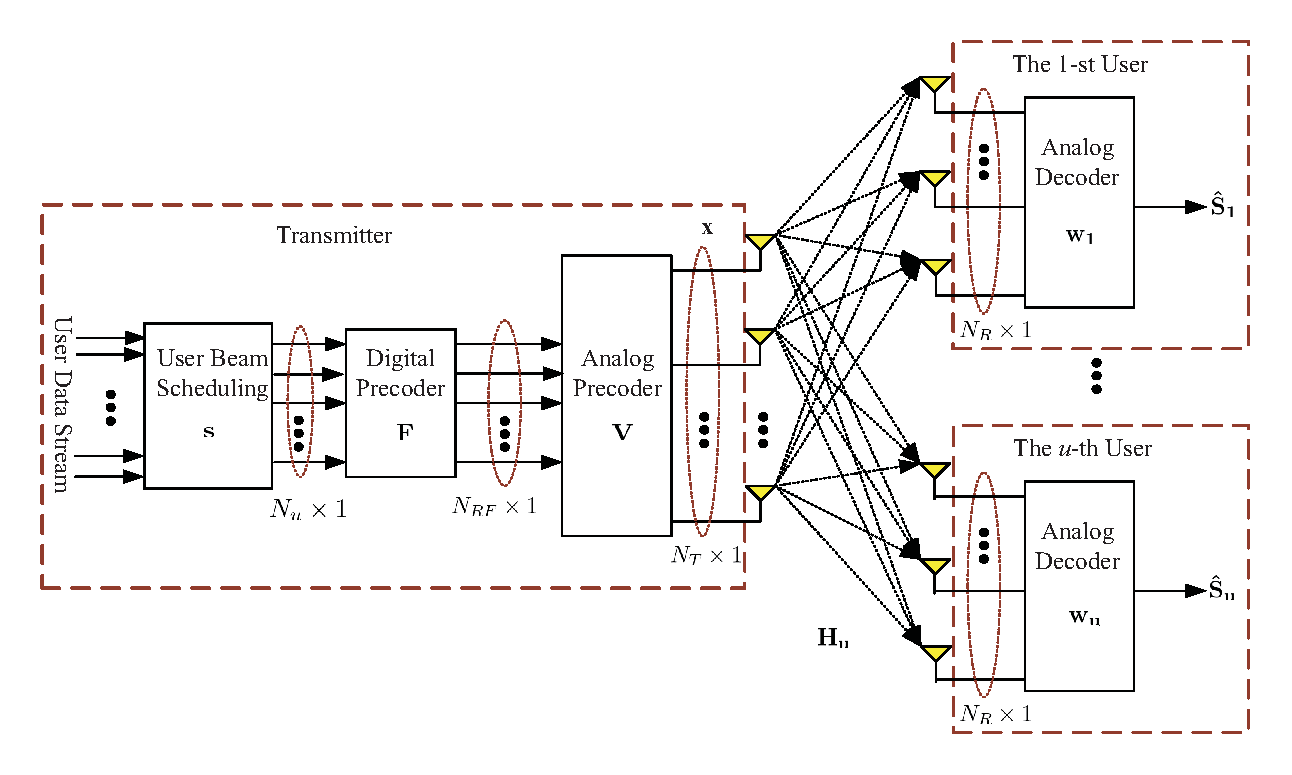
\includegraphics[scale=0.6]{Figure/SystemSchematic_new.eps}
		\caption{Block diagram of the hybrid precoding system under consideration.}\label{fig:BlockDiagram}
	\end{center}
\end{figure*}

\subsection{System Model}

We consider a multi-user mmWave MIMO system shown in \figurename{ \ref{fig:BlockDiagram}}, in which a transmitter equipped with $N_{RF}$ RF chains and $N_T$ antennas transmits $N_U$ data streams to $N_U$ receivers with $N_R$ receive antennas. Following the same assumption commonly employed in the literature \cite{alkhateeb2015limited}, we assume only one data stream is designated to each scheduled receiver. We use ${\bm s}(n)$ to denote the $n$-th block of $N_U$ data to be transmitted with $\mathbb{E}\left[\bm{ss}^H\right]=\frac{1}{N_U}\bm{I}_{N_U}$. In the sequel, we concentrate on a single block and omit the temporal index $n$ for notational simplicity.


The hybrid precoding system first multiplies ${\bm s}$ with the digital precoding matrix $\bm{F}=\left[{\bm f}_1,\cdots,{\bm f}_u,\cdots{\bm f}_{N_U}\right]$ with ${\bm f}_u$ of dimension $N_{RF}\times 1$ being the digital beamforming vector for the $u$-th user, $u=1,2,\cdots,N_U$. After that, the output signal will be multiplied by the analog precoding matrix $\bm{V}=\left[{\bm v}_1,\cdots,{\bm v}_i,\cdots,{\bm v}_{N_{RF}}\right]$ with ${\bm v}_i$ of dimension $N_T\times 1$ being the $i$-th analog beamforming vector for $i=1,2,\cdots,N_{RF}$. The resulting precoded signal $\bm x$ of dimension $N_T\times 1$  can be expressed as

\begin{equation}{\label{eq:transx1}}
{\bm x} = \bm{V}\cdot \bm{F}\cdot\bm{s}= \bm{V}\sum_{u=1}^{N_U}\bm{f}_us_u
\end{equation}

The precoded signal $\bm x$ is then broadcast to $N_U$ users. The signal received by the $u$-th user is given by

\begin{eqnarray}{\label{eq:transx2}}
{\bm y}_u &=& \bm{H}_u \bm{x} + \bm{n}_u\\
&=&\bm{H}_u \bm{V}\bm{f}_us_u+\bm{H}_u \bm{V}\sum_{\substack{i=1 \\ i\neq u}}^{N_U}\bm{f}_is_i+\bm{n}_u,
\end{eqnarray}
where $\bm{H}_u$$\in\mathbb{C}^{N_R\times N_T}$ is the MIMO channel matrix between the transmitter and the $u$-th receiver\cite{el2014spatially}. Furthermore, $\bm{n}_u$ is complex additive white Gaussian noise with zero mean and variance equal to $\sigma^2$.

Assuming the receivers are all low-cost terminals that perform analog beamforming only in decoding, the decoded signal by the $u$-th user denoted by $\hat{s}_u$ is given by
\begin{equation}{\label{eq:hats}}
\hat{s}_u = \bm{w}_u^H \bm{H}_u \bm{V} \bm{f}_{u} \bm{s} + \bm{w}_u^H \bm{\tilde{n}}_u,
\end{equation}
where ${\bm w}_u$ of dimension $N_T\times 1$ is the analog beamforming vector employed by the $u$-th receiver with the power constraint of $\|\bm{w}_u\|^2=1$ and
\begin{equation}
\bm{\tilde{n}}_u=\bm{H}_u \bm{V}\sum_{\substack{i=1 \\ i\neq u}}^{N_U}\bm{f}_is_i+\bm{n}_u.
\end{equation}
Note that the first term in Eq.~(\ref{eq:hats}) stands for the desired signal while the second term is the sum of its own receiver noise and interference from other users.

\subsection{Channel Model}
As shown in \cite{rappaport2014millimeter}, the mmWave wireless channel can be well modeled by the Saleh-Valenzuela model. Following the same approach developed in \cite{alkhateeb2015limited}, we assume that each scatter only contributes one single propagation path. As a result, the $u$-th user's channel model can been modeled as:
\begin{equation}{\label{eq:Hu}}
\bm{H}_u = \sqrt{\frac{N_{T}N_{R}}{L_{u}}}\sum_{l=1}^{L_u}\alpha_{u,l}\cdot \bm{a}_{R}(\phi^r_{u,l},\theta^r_{u,l}) \cdot\bm{a}_{T}^{H}(\phi^t_{u,l},\theta^t_{u,l}),
\end{equation}
where $L_u$ is the number of scatters of the $u$-th user's channel. Furthermore, $\alpha_{u,l}$, $\theta^r_{u,l}/\phi^r_{u,l}$ and $\theta^t_{u,l}/\phi^t_{u,l}$ are the complex path gain, azimuth/elevation angles of arrival(AoA) and azimuth/elevation angles of departure(AoD) of the $l$-th path of the $u$-th user, respectively. Finally, ${\bm a}$ is the array response vector. For an uniform planar array (UPA) of size $P\times Q$ considered in this work, the array response vector ${\bm a}$ is given by \cite{alkhateeb2015limited}
\begin{flalign}\label{eq:UPAvec1}
\bm{a}(\phi,\theta) =&\frac{1}{\sqrt{PQ}}\left[1,  e^{j\kappa d(\sin\phi \sin\theta +\cos\theta)},   \right. &&\nonumber\\
&\left. \cdots, e^{j\kappa d\left((P-1)\sin\phi \sin\theta +(Q-1)\cos\theta\right)}\right]^T,&&
\end{flalign}
where $\kappa =\frac{2\pi}{\lambda}$ is the wavenumber and $d$ is the distance between two adjacent antennas. In the sequel, our proposed schemes focus on the single-path channel model. However, extension of our proposed schemes to the multi-path scenarios is straightforward.


\subsection{Problem Formulation}
For notational simplicity, we denote by ${\bm{g}}_{u}^H$ the effective array gain of the $u$-th user with
\begin{equation}\label{eq:defgu}
{\bm{g}}_{u}^H = \bm{w}^H_u \bm{H}_u \bm{V}.
\end{equation}

Then, the channel capacity of the $u$-th user is given by
\begin{equation}\label{eq:6}
R_u(\bm{p},\bm{W},\bm{V}, \bm{F}) = \log\left(1+\frac{p_u|{\bm{g}}_{u}^H \bm{f}_u|^2}{\sum_{\substack{i=1 \\ i\neq u}}^{N_U}p_i|{\bm{g}}_{u}^H\bm{f}_i|^2+\sigma^2}\right).
\end{equation}
Subsequently, the system weighted sum-rate capacity that is a function of ${\bm V}$ and ${\bm F}$ can be computed as
\begin{equation}
R_{tot}=\sum_{u=1}^{N_U} \tau_uR_u(\bm{p},\bm{W},\bm{V}, \bm{F}).
\end{equation}
where $\bm{\tau} = \left[\tau_1, \tau_2, \cdots, \tau_{N_U}\right]$ are the corresponding weights for users.

Finally, the optimal design of the digital and analog precoding matrices as well as power allocation can be formulated as
\begin{align}\label{eq:maxsumrate}
P_1: \quad&\underset{\bm W, \bm{V},\bm F}{\text{maximize}}\quad R_{tot}(\bm{p},\bm{W}, \bm{V}, \bm{F})\\ 
\text{subject to} \quad&C_1: \|\bm{v}_{u}\|^2=1; \nonumber\\
&C_2: \|\bm{w}_{u}\|^2=1;\nonumber\\
&C_3: \|\bm{V} \bm{f}_u\|^2 \leq 1;\nonumber\\
&C_4: \sum_{u=1}^{N_U}p_{u} \leq N_U;\nonumber\\
&C_5: R_{u}\geq \lambda_{u}, \nonumber
\end{align}
where $C_1$ and $C_2$ are the analog constraints for receiver and transmitter. $C_3$ gives the power constraint for RF chains. The total transmitter power is constrained as $C_4$. Finally, $C_5$ ensures that the $u$-th user's capacity should be guaranteed not less than a certain threshold $\lambda_{u}$.

The problem $P_1$ is highly non-convex and difficult to derive a closed-form solution. In this paper, we first design the analog precoder by assuming the digital precoder as orthonormal. After solving the analog precoder, a general rank-constrained D.C programming algorithm is proposed to obtain the digital precoder such that the problem can be formulated as an iterative convex optimization problem. 

\section{Analog Beamforming Design}\label{analog}
In this section, we  assume the digital precoder is $\bm{f}_u\bm{f}_u^H = \bm{I}_{N_U}$ with uniform power allocation. Then we focus on the analog beamforming design on both transmitter and receiver sides. It's worthing to note that the proposed solution for analog and digital precoder is similar to a greedy algorithm since the analog constraint is highly non-convex and intractable.

According to the theory for infinite antenna \cite{sun2015beam}, as the number of transmit antennas $N$ goes to infinity in both transmitter and receiver, distinct array response vectors are asymptotically orthogonal, {\em i.e.}
\begin{equation}\label{Eq:assumption}
\lim_{N\rightarrow +\infty} \bm{a}^{H}(\phi^t_{k,u},\theta^t_{k,u}) \cdot\bm{a}(\phi^t_{\ell,v},\theta^t_{\ell,v})=\delta(k-\ell)\delta(u-v).
\end{equation}
However, the infinity antennas scheme is not practical. The residual interference must be considered in analog precoding design.  For multi-path channel model, we can select the transmitter paths  with maximal capacity for users.

For the array response vectors in transmitter and receiver, we denote that
\begin{align}
\mathcal{A}^T_{u} = \left[\bm{a}_{T}(\phi^t_{{u,1}},\theta^t_{{u,1}}),\cdots,\bm{a}_{T}(\phi^t_{{u,L_{u}}},\theta^t_{{u,L_{u}}})\right]
\nonumber \\
\mathcal{A}^R_{u} = \left[\bm{a}_{R}(\phi^r_{{u,1}},\theta^r_{{u,1}}),\cdots,\bm{a}_{R}(\phi^r_{{u,L_{u}}},\theta^r_{{u,L_{u}}})\right]
\end{align}

Recalling the channel model presented in Eq.~(\ref{eq:Hu}), we can asymptotically orthogonalize transmitted signals by setting the transmit analog beamforming vector for the $u$-th user as
\begin{align}\label{eq:group-scheduling}
\bm{{w}}^*_{u}, \bm{{v}}^*_{u} &=\underset{\tilde{\bm w }_{u}, \tilde{\bm v}_{u}}{\argmax}
\sum_{u=1}^{M_k}\log\left(1+ \text{SINR}\left(\tilde{\bm w}_{u}, \tilde{\bm v}_{u}\right)\right)  \\ \nonumber
\text{subject to}&\quad \tilde{\bm v}_{u}\in \mathcal{A}^T_{u},\quad \tilde{\bm w}_{u}\in \mathcal{A}^R_{u},
\end{align}
where 
\begin{equation}\label{SINR} 
\text{SINR}_u\left(\tilde{\bm w}_{u}, \tilde{\bm v}_{u}\right) = \frac{|\tilde{\bm w}^H_{u} \bm{H}_{u} \tilde{\bm v}_{u}|^2}{\displaystyle\sum_{i=1,i\neq u}^{N_U}|\tilde{\bm w}^H_{u} \bm{H}_{u}\tilde{\bm {v}}_i|^2 + 1/\gamma },
\end{equation}
where $\gamma = \frac{1}{\sigma_{u}^2}$ is the uniform SNR for each users. 

It's easy to derive the analog beamforming precoder by searching in feasible sets of $\mathcal{A}^T_{u}$ and $\mathcal{A}^R_{u}$ exhaustively.

%The denominator in Eq. \eqref{SINR} only contains the inter-cluster interference since we assume that the intra-cluster interference can be totally eliminated by digital precoder described in Section \ref{digital}. As a result, the inter-user interference can be asymptotically eliminated if a large number of beamforming antennas is employed. {\bf Simon: If inter-user interference can be asymptotically eliminated as $N\rightarrow +\infty$, the same conclusion can be also applied to the intra-cluster interference.}

%Using the analog beamforming vector in Eq.~(\ref{eq:group-scheduling}), the equivalent channel from the transmitter to user $u$ in cluster $k$ becomes $\bm{H}_{k,u}\bm{v}_{k,u}=\sqrt{N_{T}N_{R}}\alpha_{k,u}\cdot \bm{a}_{R}(\phi^r_{k,u},\theta^r_{k,u})$ and the equivalent channels to other users are all equal to zero vectors. Subsequently, the maximum ratio combing (MRC) is employed at the receiver and the resulting receive analog beamforming vector is given by:
%\begin{equation}
%\bm{w}^H_{k,u,l}=\bm{a}_{R}^{H}(\phi^r_{k,u,l},\theta^r_{k,u,l}).\\
%\label{eq:wku}
%\end{equation}
\section{General rank-constrained D.C. programming problem}\label{analogAndDigital}

\subsection{Transform Problem $P_1$ as a rank constrained D.C. Programming Problem}
After obtaining the analog precoder, a global optimization algorithm is next derived for the digital precoding design. 
Recalling the problem $P_1$, although the analog precoder is given, the function of $R_{tot}(\bm{F}, \bm{p})$ is still non-convex since $\log_2 (\cdot)$ is a concave function  while $|\cdot|^2$ is a convex function.  To settle this challenge, we form the digital precoder as
\begin{equation}
\bar{\bm{F}}_{u} = p_u\bm{f}_{u} \bm{f}_{u}^H
\end{equation}
with constraints $Rank(\bar{\bm{F}}_{u})\leq 1$ and $\bar{\bm{F}}_{u} \succeq 0$. Denoted by $\bm{\mathcal{F}} = [\bar{\bm{F}}^{(n)}_1, \bar{\bm{F}}^{(n)}_2,\cdots, \bar{\bm{F}}^{(n)}_{N_U}]$. Furthermore, the constraint $C_3$ and $C_4$ in $P_1$ can be transformed as 
\begin{equation}
\sum_{u=1}^{N_U}\bm{V} \bar{\bm{F}}_u\bm{V} ^H = \sum_{u=1}^{N_U} p_u\|\bm{V} \bm{f}_{u}\|^2\leq N_U.
\end{equation}
 
After solving the optimal $\bar{\bm{F}}_u^*$, $\bm{f}_{u}^*$ is the eigenvector corresponding to the only one non-zero eigenvalue $p_u$ of $\bar{\bm{F}}_u^*$.

Then the Equation \eqref{eq:6} can be rewritten as 
\begin{align}\label{eq:newR}
R_u(\bar{\bm{F}}_u) =& \log_2\left(1+\frac{\bm{g}_{u}^H \bar{\bm{F}}_u\bm{g}_{u}}{\sum_{\substack{i=1 \\ i\neq u}}^{N_U}{\bm{g}}_{u}^H\bar{\bm{F}}_i\bm{g}_u+\sigma^2}\right)\\
=&\log_2\left(\sum_{i=1}^{N_U}\bm{g}_{u}^H \bar{\bm{F}}_i\bm{g}_{u} + \sigma_u^2\right) \nonumber\\
&\qquad -\log_2\left(\sum_{\substack{i=1 \\ i\neq u}}^{N_U}{\bm{g}}_{u}^H\bar{\bm{F}}_i\bm{g}_u+\sigma^2 \right) \nonumber
\end{align}

Then the problem $P_1$ can be reformulated as a D.C. programming problem with a rank constraint:
\begin{align}\label{eq:maxR}
P_2: \quad&\underset{\bar{\bm{F}}}{\text{maximize}}\quad f(\bm{\mathcal{F}}) - g(\bm{\mathcal{F}})\\ \nonumber
\text{subject to} \quad&C_1: \sum_{u=1}^{N_U}\bm{V}^H \bar{\bm{F}}_u\bm{V} \leq N_U;\nonumber\\
&C_2: R_{u}\geq \lambda_{u}, u = 1,2,\cdots, N_U;\nonumber\\
&C_3: \bar{\bm{F}}_{u} \succeq 0, u = 1,2,\cdots, N_U; \nonumber\\
&C_4: Rank(\bm{\bar{F}}_{u})\leq 1, u = 1,2,\cdots, N_U, \nonumber
\end{align}
where
\begin{align}
	f(\bm{\mathcal{F}}) = \sum_{u=1}^{N_U}\tau_u\log_2\left(\sum_{i=1}^{N_U}\bm{g}_{u}^H \bar{\bm{F}}_i\bm{g}_{u} + \sigma_u^2\right),\\
    g(\bm{\mathcal{F}}) = \sum_{u=1}^{N_U}\tau_u \log_2\left(\sum_{\substack{i=1 \\ i\neq u}}^{N_U}{\bm{g}}_{u}^H\bar{\bm{F}}_i\bm{g}_u+\sigma_u^2 \right).
\end{align}
Furthermore, $C_2$ can be reformulated as
\begin{equation}
	\bm{g}_{u}^H \bar{\bm{F}}_u\bm{g}_{u} + (1-2^{\lambda_{u}}) \left( \sum_{\substack{i=1 \\ i\neq u}}^{N_U} \bm{g}_{u}^H \bar{\bm{F}}_i\bm{g}_{u} + \sigma_u^2 \right) \geq 0.
\end{equation} 
Finally, except $C_4$ constraint, a standard D.C programming problem is derived. Next, the iterative algorithm will be given to solve the problem $P_2$ by ignoring $C_4$ constraint. 

Since the problem $P_2$ still has high computational complexity, the digital precoder can be obtained by iteratively solving $\bar{\bm{F}}_u$ for $u = 1,2,\cdots, N_U$ until no improvement for next iteration.

Similar to the procedures in \cite{kha2012fast}, the iterative algorithm gives the optimal $\bar{\bm{F}}_u^{(n+1)}$ at $n$-th iteration by solving the following convex problem:
\begin{align}\label{DC}
\underset{\bar{\bm{F}}_u}{\text{maximize}}&\quad f(\bar{\bm{F}}_u) - g(\bar{\bm{F}}^{(n)}_u) - \langle \bigtriangledown g(\bar{\bm{F}}^{(n)}_u), \bar{\bm{F}}_u -  \bar{\bm{F}}_u^{(n)} \rangle\\ \nonumber
\text{subject to}& \quad C_1, C_2, C_3\quad \text{in} \quad P_2,
\end{align}
where $\langle \cdot \rangle$ denotes the inner product of two matrices, \textit{i.e.} $\langle A, B \rangle = \textbf{trace}(A^T B)$. The gradient of $g(\bar{\bm{F}}^{(n)})$ is easily given by 
\begin{equation}
	\bigtriangledown g(\bar{\bm{F}}^{(n)}_u) = \sum_{\substack{j=1 \\ j\neq u}}^{N_U}\frac{w_j/\ln 2}{\sum_{\substack{i=1 \\ i\neq j}}^{N_U} \bm{g}_{u}^H \bar{\bm{F}}_i\bm{g}_{u} +\sigma^2_j} \bm{g}_{j} \bm{g}_{j}^H.
\end{equation}
It's worthing to note that $\langle \bigtriangledown g(\bar{\bm{F}}^{(n)}_u), \bar{\bm{F}}_u -  \bar{\bm{F}}_u^{(n)} \rangle$ is a real value since $\bigtriangledown g(\bar{\bm{F}}^{(n)}_u)$ and $\bar{\bm{F}}_u -  \bar{\bm{F}}_u^{(n)}$ are all hermitian.

\subsection{General Rank Constrained Optimization Problem (RCOP)}
After obtaining the D.C. programming problem, we now consider the rank constraint $C_4$ in $P_2$. A general RCOP to optimize a convex objective subject to a set of convex constraint and rank constraint can be formulated as follows:
\begin{align}\label{eq:RCOP}
P_3: \quad& \underset{\bm{X}}{\text{minimize}}   \quad f(\bm{X}) \\
\text{subject to}& \quad \bm{X} \succeq 0;\nonumber\\
& \quad \bm{X} \in \mathcal{C}; \nonumber\\
& \quad Rank(\bm{X})\leq r,
\end{align}
where $f(\bm{X})$ is a convex function, $\mathcal{C}$ is the set of given convex constraints and $\bm{X}\in \mathbb{C}^{m\times m}$ is a general square matrix variable.

The RCOP problem can be solved by an iterative method by gradually approaching the constrained rank \cite{sun2017rank}. At each step $n$, we will solve the following semidefinite programming (SDP) problem formulated as:
\begin{align} \label{rank}
\underset{\bm{X}^{(n+1)}, e^{(n)}}{\text{minimize}}  & \quad f(\bm{X}^{(n+1)})  + w e^{(n+1)} \\
\text{subject to}& \quad \bm{X}^{(n+1)} \succeq 0;\nonumber\\
& \quad \bm{X}^{(n+1)}\in \mathcal{C}; \nonumber\\
&\quad e^{(n+1)}\bm{I}_{m-r} - \bm{U}^{(n)H} \bm{X}^{(n+1)} \bm{U}^{(n)} \succeq \bm{0};\nonumber\\
&\quad e^{(n+1)} \leq e^{(n)},\nonumber
\end{align}
where $w > 0$ is the weighting factor. $\bm{U}^{n} \in \mathbb{C}^{{m}\times (m-r)}$ is the orthonormal eigenvectors corresponding to the $n-r$ smallest eigenvalues of $\bm{X}^{(n)}$ solved at previous $(n) $-th iteration. At the first iteration where $n=0$, $e^{(0)}$ is the $(m-r)$-th smallest eigenvalue of $\bm{X}^{(0)}$. $\bm{X}^{(0)}$ is obtained via
\begin{align} \label{x0}
\underset{{\bm{X}^{(0)}}}{\text{minimize}} & \quad f(\bm{X}^{(0)}) \\
\text{subject to}& \quad \bm{X}^{(0)} \succeq 0;\nonumber\\
& \quad \bm{X}^{(0)}\in \mathcal{C}, \nonumber
\end{align}
and $\bm{U}^{(0)}$ is the eigenvectors corresponding to $n-r$ smallest eigenvalues of $\bm{X}^{(0)}$.

\section{Proposed algorithm for Rank-constrained D.C. programming problem}
\subsection{Iterative Algorithm for $P_2$}
As shown in Section \ref{analogAndDigital}, Equation \eqref{DC} is obviously a concave optimization problem.
By combining the $P_2$ and $P_3$, an iterative algorithm for rank-constrained D.C programming problem is derived. 
The optimal $g(\bar{\bm{F}}^{(n+1)})$ in the $n$-th iteration is given by solving the following convex problem:
\begin{align} \label{rankconstrainedDC}
\underset{\bar{\bm{F}}_u, e^{(n+1)}}{\text{minimize}}  & \quad  t(\bar{\bm{F}}_u, e^{(n+1)}) \\
\text{subject to}&\quad \sum_{u=1}^{N_U}\bm{V}^H \bar{\bm{F}}_u\bm{V} \leq N_U;\nonumber\\
& \quad R_{u}\geq \lambda_{u}, u = 1,2,\cdots, N_U;\nonumber\\
&\quad \bar{\bm{F}}_u \succeq 0;\nonumber\\
&\quad e^{(n+1)}\bm{I}_{N_U-1} - \bm{U}^{(n)H} \bar{\bm{F}}_u \bm{U}^{(n)} \succeq \bm{0};\nonumber\\
&\quad e^{(n+1)} \leq e^{(n)},\nonumber 
\end{align}
where
\begin{align}
 &t(\bar{\bm{F}}_u, e^{(n+1)})\nonumber\\
  = &g(\bar{\bm{F}}^{(n)}_u) + \langle \bigtriangledown g(\bar{\bm{F}}^{(n)}_u), \bar{\bm{F}}_u -  \bar{\bm{F}}_u^{(n)} \rangle  -  f(\bar{\bm{F}}_u) + w e^{(n+1)},\nonumber
\end{align}

 and $\bm{U}^{(n)}$ is the eigenvectors corresponding to $N_U-1$ smallest eigenvalues of  $\bar{\bm{F}}^{(n)}_u$.

Although the problem in Equation \eqref{rankconstrainedDC} looks very complicated, it's a standard convex optimization problem and can be solved via available convex software packages, such as CVX \cite{cvx}.

The proposed iterative algorithm can be summarized as \textbf{Algorithm 1}. In each iteration, we solve a D.C programming problem and update the variable $\bar{\bm{F}}^{(n)}_u$. If the weighted sum-rate capacity $s^{(n)}$ can be no longer improved, the digital precoder $\bar{\bm{F}}^{(n)}_{u+1}$ of $(u+1)$-th user is then optimized successively. The iteration will stop if no any improvement for $\bm{\mathcal{F}}$.

\begin{algorithm}[h] 		
	\caption{Iterative Rank-constrained D.C. Problem}
	\label{beam_cluster}
	\begin{algorithmic}
		\REQUIRE  \quad
		\STATE Effective channel: $\bm{g}_{1},\bm{g}_{2},\cdots,\bm{g}_{N_U}$; 
		\STATE Random initialization matrices of $\bar{\bm{F}}_u^{(0)}$, $u = 1,2,\cdots, N_U$;
		\STATE The initialization information: $s$, $s'$, $t^{(0)}$, $t^{(1)}$, $\epsilon$;
		\STATE The initialization value by solving Equation \eqref{x0}: $\bm{U}^{(0)}, e^{(0)}$
		%\STATE $\bm{\mathcal{I}} \leftarrow \mathcal{I}_1$ and ${\mathcal X}\setminus x^*$;
		\ENSURE   
	\end{algorithmic}		
	\begin{algorithmic}[1]
		\WHILE{$|(s' - s)/s|\leq \epsilon$}
		\STATE Update $s$: $s = s'$
		\FOR{$0\leq u \leq N_U$}
		\STATE $n = 0$
		\WHILE{$|(t^{(n+1)} - t^{(n)})/t^{(n)}|\leq \epsilon$}
       	\STATE Obtain the optimal value $t^{(n+1)}$ of objective function and $\bar{\bm{F}}^{(n+1)}_u, e^{(n+1)}$ in Equation \eqref{rankconstrainedDC}
       	\STATE Update $\bm{U}^{(n)}$ from $\bar{\bm{F}}^{(n+1)}_u$ via eigenvalue decomposition and set $n = n+1$
       	\ENDWHILE
		\ENDFOR
		\STATE Update $s'$: $s' = t^{(n+1)}$
		\ENDWHILE
		\STATE Outputs: $\bm{\mathcal{F}}^* =[\bar{\bm{F}}^{(n)}_1, \bar{\bm{F}}^{(n)}_2,\cdots, \bar{\bm{F}}^{(n)}_{N_U}] $.
	\end{algorithmic}
\end{algorithm}

\subsection{Convergence of Proposed Iterative Algorithm}
In the following, we provide the convergence analysis of the proposed iterative algorithm for solving the rank-constrained D.C. programming problem.

As the function $g(\bar{\bm{F}}_u)$ is concave, its gradient $\bigtriangledown g(\bar{\bm{F}}_u)$ is also its super-gradient, therefore
\begin{equation}
	g(\bar{\bm{F}}_u)\leq g(\bar{\bm{F}}^{(n)}_u) + \langle \bigtriangledown g(\bar{\bm{F}}^{(n)}_u), \bar{\bm{F}}_u -  \bar{\bm{F}}_u^{(n)} \rangle.
\end{equation}

Since $ e^{(n+1)} \leq e^{(n)}$ and $\bar{\bm{F}}_u^{(n)}$ is feasible to Equation \eqref{rankconstrainedDC}, it follows
\begin{align}
&g(\bar{\bm{F}}^{(n+1)}_u)  - f(\bar{\bm{F}}^{(n+1)}_u)  + e^{(n+1)} \\
\leq&g(\bar{\bm{F}}^{(n)}_u) + \langle \bigtriangledown g(\bar{\bm{F}}^{(n)}_u), \bar{\bm{F}}_u -  \bar{\bm{F}}_u^{(n)} \rangle - f(\bar{\bm{F}}_u) + e^{(n)}.\nonumber\\
\leq &g(\bar{\bm{F}}^{(n)}_u)  - f(\bar{\bm{F}}^{(n)}_u)  + e^{(n)}, \nonumber
\end{align}
which shows that the solution $\bar{\bm{F}}^{(n+1)}_u$ is always better than or equal to the previous solution $\bar{\bm{F}}^{(n)}_u$. Obviously, this inequality will also hold if the variable $\bar{\bm{F}}_u$ changes to $\bar{\bm{F}}_{u+1}$.

\section{Simulation Results}
In this section, we will use computer simulation to show the effectiveness of proposed rank-constrained D.C. programming algorithm. Unless specified otherwise, we consider a transmitter equipped with a $6\times 6$ UPA ({\em i.e.} $N_T=36$) and $N_U=4$ users each equipped with a $4\times 4$ UPA ({\em i.e.} $N_R=16$). The number of paths is set as $L_{u} = 4$. We consider the azimuth AoAs/AoDs uniformly distributed over $[0, 2\pi]$ while the elevation AoAs/AoDs uniformly distributed over $[-\pi/2, \pi/2]$, respectively. The wights are given as   $\bm{\tau} = [1.5,1.5,0.5,0.5]$. 
\begin{figure}[ht]
	\begin{center}
		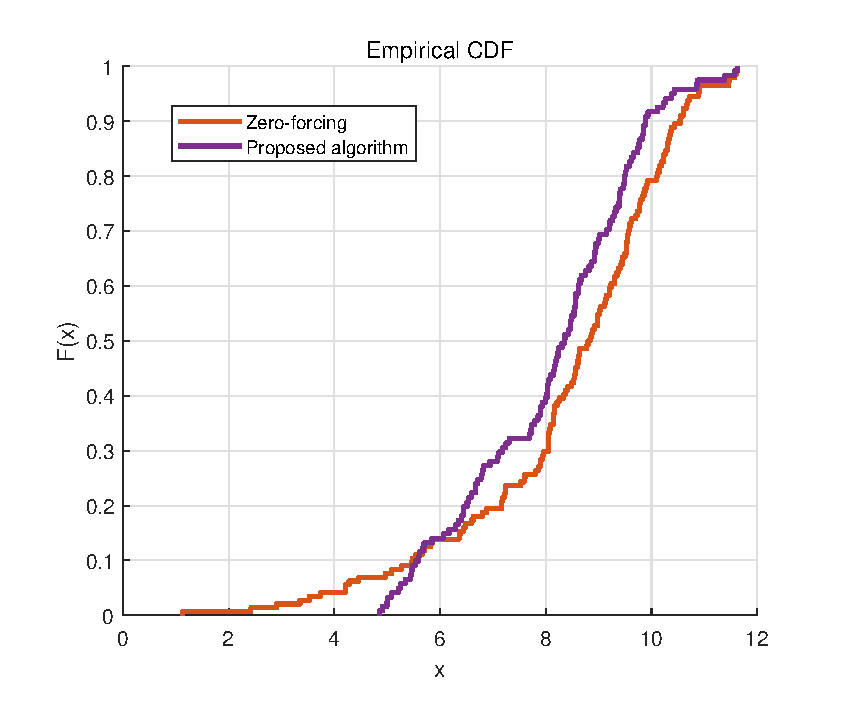
\includegraphics[width=3.5in]{Figure/ZF_VS_DC.eps}
		\caption{CDF of capacity.}\label{fig:CDF}
	\end{center}
\end{figure}

Fig. \ref{fig:CDF} compares the CDF of capacities between zero-forcing and proposed algorithm. The additive Gaussian noise is set as $-10$ dB. The figure confirms $C_5$ constraint in $P_1$ as the threshold $\lambda_{u} = 5 $ bps/Hz.

\begin{figure}[ht]
	\begin{center}
		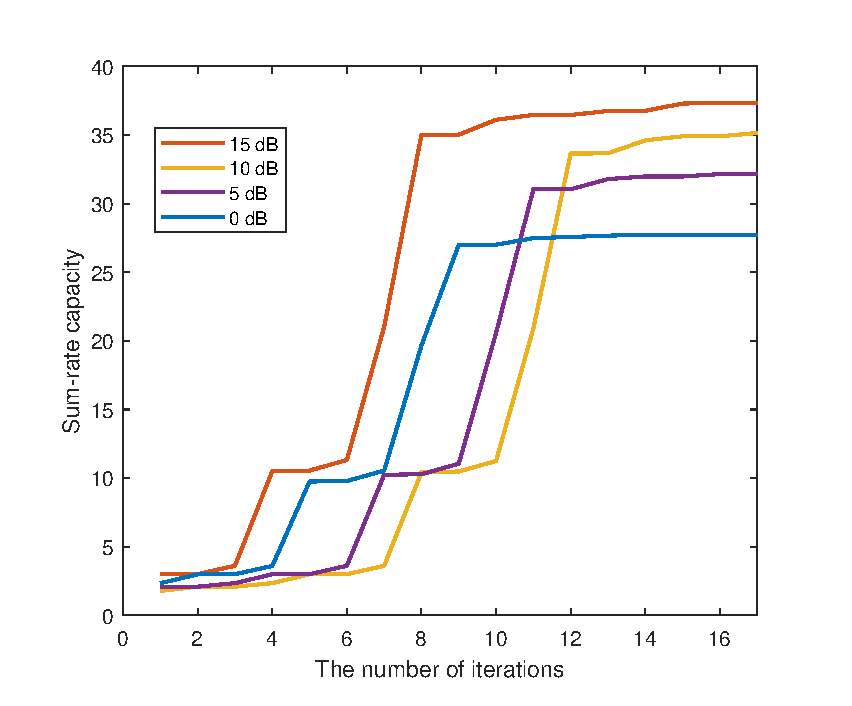
\includegraphics[width=3.5in]{Figure/convergence.eps}
		\caption{The proof of convergence and monotonicity.}\label{fig:mono}
	\end{center}
\end{figure}

Next, the monotonicity and convergence of the proposed iterative algorithm are shown in Fig. \ref{fig:mono} for different given SNR from $0-15$ dB.

\bibliography{REFDCprecode}
\bibliographystyle{IEEEtran}


%\EOD

\end{document}
